\documentclass{standalone}
\usepackage{tikz}
\usepackage{tikz-qtree}
\usepackage[makeroom]{cancel}
\usetikzlibrary{fit}

% ОПИСАНИЕ: модификация старого алгоритма tree overlap чтобы покрывать все деревья 
\begin{document} 
	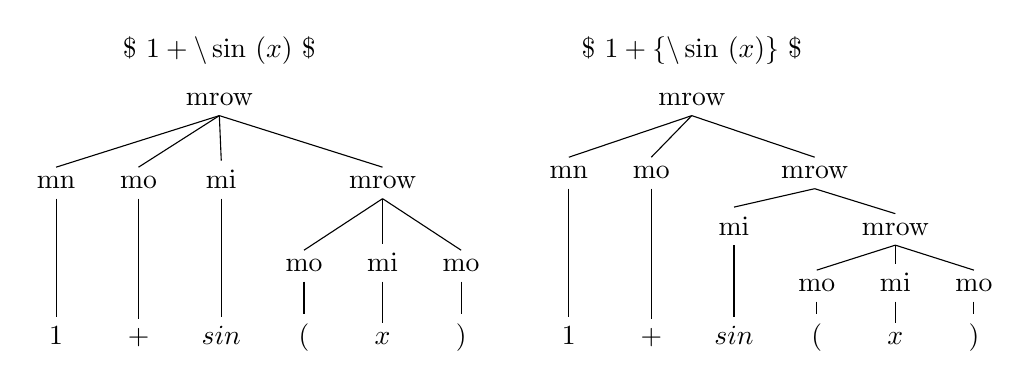
\begin{tikzpicture}[sibling distance=9.5pt]
	\tikzset{frontier/.style={distance from root=7.2\baselineskip}}
	\node (x) at (0,0.7) {$ \$~1 + \texttt{\textbackslash}\sin~(x)~\$$};
	    \Tree [.mrow
	            [.mn $1$ ] 
	            [.mo $+$ ]
	            [.mi $sin$ ]
	            [.mrow 
	            	[.mo $($ ]
	            	[.mi $x$ ]
	            	[.mo $)$ ]
	            ]
	          ]
	    \begin{scope}[xshift=6cm]
	\tikzset{level 1/.style={level distance=2.2\baselineskip}}
	\tikzset{level 2+/.style={level distance=1.7\baselineskip}}
	\node (x) at (0,0.7) {$ \$~1 + \{\texttt{\textbackslash}\sin~(x)\}~\$$};
	    \Tree [.mrow
	            [.mn $1$ ] 
	            [.mo $+$ ]
	            [.mrow
	            	[.mi $sin$ ]
	            	[.mrow 
	            		[.mo $($ ]
	            		[.mi $x$ ]
	            		[.mo $)$ ]
	            	]
	            ]
	          ]
	    \end{scope}
	\end{tikzpicture}
\end{document} 